\documentclass[conference]{IEEEtran}
\IEEEoverridecommandlockouts
% The preceding line is only needed to identify funding in the first footnote. If that is unneeded, please comment it out.
\usepackage{cite}
\usepackage{amsmath,amssymb,amsfonts}
\usepackage{algorithmic}
\usepackage{graphicx}
\usepackage{textcomp}
\usepackage{xcolor}
\usepackage{multirow}
\usepackage{subcaption}
\usepackage{float}
% Added for plotting with tikz/pgfplots used in the figure environments
\usepackage{tikz}
\usepackage{pgfplots}
\pgfplotsset{compat=1.18}
\def\BibTeX{{\rm B\kern-.05em{\sc i\kern-.025em b}\kern-.08em
    T\kern-.1667em\lower.7ex\hbox{E}\kern-.125emX}}
\begin{document}

\title{Enhancing Pedagogical Feedback Quality of Large Language Models via Learning Analytics in a Kanban-Based Platform for Student Self-Regulated Learning Support}

\author{
\IEEEauthorblockN{1\textsuperscript{st} \textit{Qornain Aji}}
\IEEEauthorblockA{\textit{Department of Electrical and}\\
\textit{Information Engineering} \\
\textit{Universitas Gadjah Mada}\\
Yogyakarta, Indonesia\\
qornain.aji@mail.ugm.ac.id}
\and
\IEEEauthorblockN{2\textsuperscript{nd} \textit{Indriana Hidayah}}
\IEEEauthorblockA{\textit{Department of Electrical and}\\
\textit{Information Engineering} \\
\textit{Universitas Gadjah Mada}\\
Yogyakarta, Indonesia\\
indriana.h@ugm.ac.id}
\and
\IEEEauthorblockN{3\textsuperscript{rd} \textit{Syukron Abu Ishaq A.}}
\IEEEauthorblockA{\textit{Department of Electrical and}\\
\textit{Information Engineering} \\
\textit{Universitas Gadjah Mada}\\
Yogyakarta, Indonesia\\
syukron.abu@ugm.ac.id}
}

\maketitle

\begin{abstract}
% This document is a model and instructions for \LaTeX.
% This and the IEEEtran.cls file define the components of your paper [title, text, heads, etc.]. *CRITICAL: Do Not Use Symbols, Special Characters, Footnotes, 
% or Math in Paper Title or Abstract.
This study aims to enhance the quality of pedagogical 
feedback generated by Large Language Models (LLMs) to 
support student Self-Regulated Learning (SRL), addressing 
the scalability crisis of human expert feedback. The 
enhancement focuses on three core functions such as 
feedback, motivation, and appreciation. A comparative 
experimental method was employed without fine-tuning, 
evaluating various Context Engineering schemes enriched 
with Learning Analytics (LA) on two models: Llama 3.1 8B 
and Llama 3.3 70B. Evaluation was quantitative (BERTScore, 
BARTScore, LLM-as-a-Judge) and qualitatively validated by 
educational psychology experts.

Results indicate that the effectiveness of the enhancement 
significantly depends on the model size. The smaller model 
(8B) achieved the highest performance increase with complex 
context (ReAct + LA), suggesting a reliance on rich, structured 
guidance to compensate for its internal limitations. 
Conversely, the larger model (70B), despite having a superior 
Baseline performance, showed degraded performance when given 
overly complex context. The best-performing model (Llama 8B 
with ReAct + LA) was validated by human experts as "Usable 
with minor revision". The study concludes that LA-enriched 
context engineering is an effective, practical, and computationally 
efficient strategy for improving pedagogical feedback, particularly 
for smaller LLMs.

% Keywords: Large Language Model, Self-Regulated Learning, Learning 
% Analytics, Context Engineering, Pedagogical Feedback.
\end{abstract}

\begin{IEEEkeywords}
Large Language Model, Self-Regulated Learning, Learning Analytics, 
Context Engineering, Pedagogical Feedback
\end{IEEEkeywords}

\section{Introduction}
% This document is a model and instructions for \LaTeX.
% Please observe the conference page limits. 
The current landscape of higher education demands that s
tudents possess the ability to learn independently. However, 
many are unprepared to face these demands. This creates a 
serious gap in \textit{Self-Regulated Learning} (SRL) skills, 
which can hinder learning success and disrupt equitable access 
to education \cite{liu2025srl, xiao2019relationships}. This challenge 
is exacerbated by the digital technologies that characterize modern 
learning. While offering flexibility, these technologies also present 
significant distractions and require greater self-discipline 
\cite{chitra2022srl}. Institutional failure to provide adequate 
support for SRL development is not merely an academic issue; it is a 
social issue that impacts students' long-term career prospects and the 
overall effectiveness of the education system \cite{liu2025srl}. 
% ------------------------------------------------

To address the SRL gap, Zimmerman proposed a framework encompassing 
the phases of planning (\textit{forethought}), execution 
(\textit{performance}), and self-reflection (\textit{self-reflection}), 
wherein SRL is a combination of cognitive, motivational, and 
behavioral strategies \cite{liu2025srl, akdeniz2022srl}. 
Individuals with effective self-regulation capabilities are 
formed through goal setting, strategy planning, active 
self-monitoring, and thoughtful self-evaluation. A substantial 
body of research confirms a strong relationship between these 
skills and academic achievement \cite{liu2025srl, xiao2019relationships}. 
However, their development is often hindered by personal, 
contextual, and social factors, ranging from poor time 
management and digital distractions to low metacognitive 
awareness. Metacognition itself refers to the knowledge, 
awareness, and regulation of one's own thinking, playing a 
crucial role in building students' awareness of their 
learning processes \cite{zimmerman2009selfregulation}. 
These barriers necessitate structured interventions to guide 
students through this complex process \cite{chitra2022srl, 
10.3389/feduc.2024.1418297}.

The most effective traditional method for developing SRL 
skills is personalized feedback from human experts. 
High-quality feedback that focuses not only on the quantity 
of completed tasks but also on the student's learning process 
and self-regulation serves as a powerful catalyst for 
improvement [15, 16]\cite{10.3389/fpsyg.2022.1027266, Bock14032024}. 
However, this "gold standard" faces a scalability crisis; increasing 
student numbers and diverse support needs make the personalized 
guidance model difficult to implement on a large scale. This is 
reinforced by studies showing that budgetary pressures drive larger 
class sizes, thereby severely limiting personal interaction between 
lecturers and students \cite{schaffer2017automating, pardo2019using}. 
This creates an urgent need for innovative technology-based solutions 
that can complement human expertise.

One such technology is the use of \textit{Large Language Models} 
(LLMs). LLMs can be employed as virtual tutors capable of providing 
fast and consistent feedback. LLMs have been utilized in various 
educational research contexts with diverse breakthroughs. Recent 
findings show that when LLMs are used for assessment and feedback, 
\textit{artificial intelligence} (AI) tends to be generous in 
grading, resulting in scores higher than those given by human 
experts. Meanwhile, peer and lecturer assessments tend to be 
lower and more aligned with student performance. AI feedback is 
often structured but still requires human expert oversight to 
remain pedagogically relevant, leading to the recommendation of 
a hybrid approach (combining AI and human experts) 
\cite{Usher2025GenAIAssessments}. A hybrid approach is 
recommended as it can combine the speed and scalability of AI 
with the contextual mastery, empathetic understanding, and 
pedagogical nuances of human assessment 
\cite{Usher2025GenAIAssessments}. This recommendation underscores 
that LLM responses still require expert supervision to be relevant. 
On the other hand, efforts to standardize AI-tutor evaluation 
indicate that although current models like GPT-4 are strong in 
answering questions, they tend to provide answers to students 
too quickly and lack process guidance. This fact suggests that 
LLMs are not yet ideal as tutors and cannot yet replace human 
experts in assessing pedagogical quality 
\cite{Maurya2025UnifyingAITutorEvaluation}.

Therefore, this thesis focuses on improving the performance 
quality of LLM responses as feedback providers to approach 
the quality of human experts, both quantitatively and 
qualitatively. This improvement is executed through an 
evaluation framework that combines human expert references as 
\textit{ground truth} with quality assessments evaluating 
relevant pedagogical dimensions \cite{Usher2025GenAIAssessments, 
Maurya2025UnifyingAITutorEvaluation}. 
% ------------------------------------------------- 
To support this measurement process, this thesis utilizes 
structured learning process traces. Student learning data, 
presented in the form of a Kanban board, is used solely as 
an operational tool to organize and extract process data 
(card movement, checklists, completion time) that can be 
mapped to SRL phases (planning-monitoring-reflecting) 
\cite{strickroth2022kanban}. The use of the Kanban board 
serves only as a data enrichment instrument to ensure the 
evaluation and improvement of LLM feedback quality proceeds 
more purposefully. In this research, as explained in the 
subsequent chapter, the focus of novelty lies in the series 
of evaluations and refinements of the LLM \textit{prompts}. 
This research aims to improve three main pedagogical 
functions—feedback, motivational support, and appreciative 
support—with the practical goal of matching human expert 
quality on quantitative metrics while simultaneously meeting 
qualitative quality standards \cite{10.3389/fpsyg.2022.1027266, 
Bock14032024, Usher2025GenAIAssessments, 
Maurya2025UnifyingAITutorEvaluation}. By comparing LLM 
outputs with expert specialists, this study assesses the 
improvement in LLM performance for consideration as a 
massive yet personalized complementary pedagogical agent 
for students.

\section{Related Works}
% \subsection{Improving LLM Feedback with \textit{Direct Preference Optimization} (DPO)}
Woodrow, Koyejo, and Piech \cite{woodrow2025dpo_feedback} address 
the \textit{Feedback Alignment Challenge}, namely the tendency 
of LLM-generated feedback to be generic and misaligned with 
course-specific rigor, terminology, and instructor preferences. 
They propose \textit{Direct Preference Optimization} (DPO) with 
teachers in the loop, where TAs select or edit preferred outputs 
from model pairs during grading, producing preference data that 
enables fine-tuning without a reward model as in RLHF. Their 
three-stage pipeline (preference collection, DPO training, inference) 
forms a self-improving system that increasingly aligns with 
course expectations across assignments. Using Llama~3.1~8B 
fine-tuned with HuggingFace DPOTrainer, they conducted controlled 
blind evaluations with experts and real deployments in large 
university courses, supported by automated assessment frameworks 
(e.g., Scarlatos et al.~\cite{scarlatos2024validity}). Results 
show that DPO outperformed GPT-4o in preference (56.8\% vs.\ 40.2\%), 
insightfulness, correctness, tone positivity, and consistency, 
though GPT-4o remained stronger in conciseness and suggestions. 
Deployment demonstrated feasibility at scale and potential for 
fairness monitoring, positioning DPO as a practical strategy for 
course-aligned AI feedback generation.

% \subsection{Improving LLM \textit{Feedback} with \textit{Prompt Engineering}}
Jacobsen and Weber \cite{jacobsen2025promises} examine how prompt 
quality shapes LLM feedback effectiveness in higher education and 
compare LLM-generated feedback with novice and expert human 
feedback. They develop a theory-based prompt manual covering 
role/context specification, mission clarity, instructional 
logic, and domain specificity, then craft low-, medium-, and 
high-quality prompts to systematically test prompt effects using 
ChatGPT-4. Across a geometry learning task involving typical 
student misconceptions, 60 LLM outputs were coded with 
pedagogical criteria (e.g., concreteness, activation, empathy, 
specificity) and compared with feedback written by preservice 
teachers and experts using the same high-quality prompt. Results 
show that only high-quality prompts reliably produce strong 
LLM feedback; LLMs outperform novices in most categories and 
even exceed experts in explanation, guiding questions, and 
specificity, while affective dimensions remain mixed. 
Efficiency gains were substantial, as ChatGPT-4 produced 
dozens of feedback instances in the time an expert crafted 
one. The authors highlight the necessity of structured prompt 
design training for educators and note limitations such as 
hallucination risks and the need to test student perceptions 
and transferability across contexts.

% \subsection{\textit{Reinforcement Learning from Human Feedback} (RLHF) for Response Quality Improvement}
Ouyang et al.\ \cite{ouyang2022traininglanguagemodelsfollow} 
introduce an RLHF pipeline to align language models with user 
intent, addressing limitations of large pretrained models that 
may generate incorrect, unhelpful, or unsafe outputs despite 
high linguistic proficiency. Their three-stage approach 
includes supervised fine-tuning on human demonstrations, 
reward model (RM) training from human comparisons, and policy 
optimization with PPO using RM predictions as rewards. Drawing 
on prompts from labelers and real API usage, they train reward 
models (initialized from GPT-3 6B) and RLHF policies with careful 
stability controls (KL penalties, learning rate warmup, single-epoch 
RM training to avoid overfitting). The resulting InstructGPT models 
show substantial alignment gains: the 1.3B RLHF model is 
preferred over the much larger GPT-3 175B baseline, while 
exhibiting improved truthfulness, reduced toxicity, and minimal 
regression on NLP benchmarks. The study demonstrates that human 
feedback alignment can outperform mere parameter scaling, while 
acknowledging remaining errors and offering a blueprint for 
instruction-following models widely adopted today.

% \subsection{Self-Regulation in LLM-Based Programming Education with \textit{Learning Analytics}}
Li and Ma \cite{li2025designaipoweredtoolselfregulation} propose 
CodeRunner Agent, an AI-powered system integrated into Moodle to 
support self-regulated learning (SRL) in programming education, 
addressing limitations of external LLM tools that lack course context 
and produce feedback disconnected from curricula or student 
behavioral data. The system combines a lecture viewer, CodeRunner 
execution/grading, and xAPI-based learning analytics to capture 
rich process data. Its pedagogical foundation is the PPESS model 
(Planning, Program creation, Error correction, Self-monitoring, 
Self-reflection), allowing students to request AI help targeted 
to their current SRL phase. Two context engines drive feedback 
relevance: LACE (Learning Analytics Context Engine) summarizes 
engagement and performance patterns from logs, while KCE (Knowledge 
Context Engine) manages curated course materials, concepts, 
solution structures, and typical errors. These engines inject 
SRL and knowledge-context cues into prompts to ensure feedback 
aligns with curriculum goals while avoiding spoon-feeding. The 
paper presents a design and planned evaluations—including 
behavioral analytics and qualitative assessments—to validate 
impact on SRL, code performance, and pedagogical safety, 
highlighting the feasibility of an end-to-end, context-aware, 
LMS-native AI support system.

% \subsection{\textit{Real-time} Dashboard for Kanban-Based Classroom Orchestration}
Strickroth, Kreidenweis, and Götzfried propose a real-time, 
networked extension of AgileBoard4Teaching to address 
orchestration challenges in collaborative, task-based 
classrooms where teachers struggle to monitor diverse group 
progress simultaneously. Their client-server system includes
 an authoring mode for task setup, a Kanban interface for 
 students, and a teacher dashboard that displays per-group 
 progress summaries, pending reviews, hand-raise signals, 
 timers, messaging, and live synchronization via WebSockets, 
 with storage handled through Java Servlets and MariaDB. Two 
 evaluations were conducted: a field study with 8th-grade 
 students using a within-subjects comparison of offline 
 versus networked versions, and a simulation study with 
 experienced teachers. Findings show strong preference for 
 the networked system, improved workflow fluency, high 
 usability scores (student SUS 84, teacher SUS 92), and high 
 engagement observed in interaction logs; the simulation 
 study also yielded positive reception despite some bugs. 
 Teachers valued real-time monitoring and ease of scaling 
 boards, suggesting refinements for large-class readability 
 and analytics features. Overall, the study demonstrates the 
 feasibility and pedagogical value of real-time dashboards 
 for classroom orchestration.

In light of the comparative review, this study adopts a 
pragmatic hybrid approach that prioritizes resource-efficient 
context alignment, namely high-quality prompt engineering 
and the injection of learning-analytics signals from Kanban 
process data, while maintaining strong pedagogical oversight. 
Instead of relying on costly full-model retraining, the method 
enriches teacher-authored prompts with contextual features such 
as task states, time-on-task, and review requests to make LLM 
feedback more course and SRL aware. Preference-based fine-tuning 
approaches (e.g., DPO or RLHF) are considered only as long-term 
options when sufficient preference labels and computational 
resources are available. Evaluation will combine quantitative 
comparisons of LLM outputs against expert-based rubrics and 
automated metrics with qualitative expert judgment to ensure 
pedagogical soundness. The accompanying real-time dashboard 
further enables continuous monitoring and iterative refinement 
of prompts and contextual cues. Altogether, this design aims 
to deliver a scalable, low-cost pipeline that leverages 
prompt/context engineering and learning-analytics signals to 
generate specific, actionable, and pedagogically aligned 
feedback while keeping instructors firmly in the loop.

% \subsection{Maintaining the Integrity of the Specifications}

% The IEEEtran class file is used to format your paper and style the text. All margins, 
% column widths, line spaces, and text fonts are prescribed; please do not 
% alter them. You may note peculiarities. For example, the head margin
% measures proportionately more than is customary. This measurement 
% and others are deliberate, using specifications that anticipate your paper 
% as one part of the entire proceedings, and not as an independent document. 
% Please do not revise any of the current designations.

\section{Methodology}
The research was conducted through several stages. The research
starting with a comprehensive literature review to understand
the current methods for improving LLM performance in producing
higher feedback quality. This review covered techniques such as
Reinforcement Learning from Human Feedback (RLHF), Direct Preference
Optimization (DPO), and Context Engineering, as well as the use of
Learning Analytics (LA) to enrich context for LLMs. The literature
review also examined the pedagogical aspects of feedback in
supporting Self-Regulated Learning (SRL) and the use of Kanban-based
platforms for organizing student learning processes.
After identifying the research gap, the next step involved selecting
various LLM models and prompting techniques for evaluation.

% Before you begin to format your paper, first write and save the content as a 
% separate text file. Complete all content and organizational editing before 
% formatting. Please note sections \ref{AA}--\ref{SCM} below for more information on 
% proofreading, spelling and grammar.

% Keep your text and graphic files separate until after the text has been 
% formatted and styled. Do not number text heads---{\LaTeX} will do that 
% for you.

\subsection{Tools}\label{AA}
The tools used in this final project consist of both 
hardware and software as supporting resources. The 
hardware employed is personally owned. The function 
of these hardware and software tools is to facilitate 
code development, chatbot implementation, quantitative 
and qualitative evaluations, as well as dataset collection. 
The following is the list of tools used in this research 
project.

\begin{enumerate}
    \item \textbf{Hardware:}
        \begin{itemize}
            \item MacBook Pro 14 inch: M1 Pro 10-core processor @ 3.2 GHz
            \item Internal GPU: M1 Pro 16-core GPU
            \item Neural Engine: 32-core
            \item RAM: 16 GB Unified Memory (200 GB/s memory bandwidth)
            \item Storage: 1 TB internal Solid State Drive (macOS 26 Tahoe)
        \end{itemize}
        \item \textbf{Software:}
            \begin{itemize}
                \item Visual Studio Code version 1.105.1: Used for writing and managing code.
                \item Google Docs: Web-platform for drafting questionnaires, performing revisions, and documenting discussion results.
                \item Google Sheets: Web-platform that is used to visualize and manage student Kanban learning data to share with experts for completion and assessment, facilitating collaboration and metric collection.
                \item Anaconda: Python package and virtual environment manager used during development.
            \end{itemize}
        \item \textbf{Key Libaries and Frameworks:}
            \begin{itemize}
                \item \texttt{Python 3.12.7}: Primary programming language for developing the LLM-based chatbot.
                \item \texttt{LangChain}: Framework for building LLM applications, providing modular components for prompt orchestration, data flows, and external data integration.
                \item \texttt{LangGraph}: An extension of LangChain for constructing more complex application flows as graphs.
                \item \texttt{bert\_score}: Quantitative evaluation framework to measure semantic similarity (Precision, Recall, F1) between model responses and ground truth.
                \item \texttt{BARTScorer}: Alternative quantitative evaluation framework (using mBART) to compute F1, Precision, and Recall based on token log-probabilities.
                \item \texttt{pandas}: Library for data manipulation, aggregation, and presentation of evaluation summary tables (e.g., BARTScore and GPT-4o Judge).
            \end{itemize}
\end{enumerate}

\subsection{Datasets Creation}
This study necessitated a specialized dataset 
capable of reflecting student learning processes 
within a \textbf{Kanban-based learning analytics platform}, 
while simultaneously possessing high-quality pedagogical ground truth. 
Due to the unavailability 
of public datasets meeting these specific criteria, 
a comprehensive methodology for \textbf{synthetic data generation} 
was designed. The objective was to 
produce a realistic and diverse dataset comprising 
two main components such as \textbf{student digital trace data in JSON format} 
representing Kanban board activities, 
and \textbf{aligned human expert feedback}.

The data generation process began with a deconstruction 
of the \textbf{Gamatutor} platform's database schema to identify 
key attributes reflecting SRL processes, 
such as column movements, timestamps, 
and checklist progress. To capture a broad spectrum of 
student engagement, five distinct behavioral profiles 
were defined: \textbf{``Lazy''}, \textbf{``Slightly Lazy''}, \textbf{``Average''}, 
\textbf{``Diligent''}, and \textbf{``Very Diligent''}. These profiles 
were operationalized into strict case study rules 
governing variables like total card count and 
checklist completion percentages. The content 
domain was restricted to \textbf{Object-Oriented 
Programming (OOP)} with five specific subtopics.

These structural and behavioral constraints were 
transformed into highly structured prompts using 
advanced engineering techniques, including 
\textbf{Role-play}, \textbf{Few-shot (providing JSON examples)}, 
and \textbf{Chain-of-Thought (CoT)} to guide the LLM's 
reasoning. Using the \textbf{ChatGPT-5 Thinking model}, 
\textbf{40 unique Kanban datasets} 
were generated. The following table summarizes the 
distribution of datasets across the defined behavioral profiles
is shown in Table \ref{tab:dataset_summary}.
\begin{table}[htbp]
% \begin{table}[]
\caption{Dataset summary by behavioral profile}
\begin{center}
\begin{tabular}{|l|c|}
\hline
Behavioral Profile & Total Datasets \\
\hline
Lazy & 5 \\
Slightly Lazy & 10 \\
Average & 10 \\
Diligent & 10 \\
Very Diligent & 5 \\
\hline
\textbf{Total} & \textbf{40} \\
\hline
\end{tabular}
\label{tab:dataset_summary}
\end{center}
\end{table}

Subsequently, to establish the \textbf{ground truth}, 
the raw \textbf{JSON data} was transformed into 
\textbf{human-readable tabular formats}. These tables 
were presented to \textbf{three human experts} 
(university lecturers), who provided 
\textbf{structured pedagogical feedback} covering 
three primary functions: \textbf{feedback, motivation}, 
and \textbf{appreciation}. This collection of expert 
feedback served as the definitive \textbf{ground truth} 
for evaluating the LLM agents in this study.




% \begin{itemize}
%     \item Use either SI (MKS) or CGS as primary units. (SI units are encouraged.) English units may be used as secondary units (in parentheses). An exception would be the use of English units as identifiers in trade, such as ``3.5-inch disk drive''.
%     \item Avoid combining SI and CGS units, such as current in amperes and magnetic field in oersteds. This often leads to confusion because equations do not balance dimensionally. If you must use mixed units, clearly state the units for each quantity that you use in an equation.
%     \item Do not mix complete spellings and abbreviations of units: ``Wb/m\textsuperscript{2}'' or ``webers per square meter'', not ``webers/m\textsuperscript{2}''. Spell out units when they appear in text: ``. . . a few henries'', not ``. . . a few H''.
%     \item Use a zero before decimal points: ``0.25'', not ``.25''. Use ``cm\textsuperscript{3}'', not ``cc''.)
% \end{itemize}

\subsection{Model Selections}
This study utilizes two distinct models from the Llama family, 
accessible via the Groq API, Llama 3.1 8B Instant and 
Llama 3.3 70B Versatile, to generate pedagogical feedback 
supporting student SRL. The selection of these specific 
LLMs was driven by several strategic considerations rather 
than being the primary object of the research itself.

Firstly, the decision was significantly influenced by 
financial and computational resource constraints, a valid 
justification in academic educational research. The Groq 
API provides these models at cost-effective rates, enabling 
broader accessibility for research purposes \cite{groq_pricing}. The specific 
pricing and specifications for the models used, alongside 
others in the ecosystem, are detailed in Table \ref{tab:model_pricing}.

\begin{table}[htbp]
\caption{Groq API Model Pricing and Specifications}
\centering
\scriptsize
\resizebox{\columnwidth}{!}{%
\begin{tabular}{|l|c|c|c|}
\hline
\textbf{Model (Configuration)} & \textbf{TPS} & \textbf{Input (\$/1M tokens)} & \textbf{Output (\$/1M tokens)} \\
\hline
\begin{tabular}[t]{@{}l@{}}Llama 4 Scout\\(17Bx16E)\end{tabular} & 594 & \$0.11 & \$0.34 \\
\begin{tabular}[t]{@{}l@{}}Llama 4 Maverick\\(17Bx128E)\end{tabular} & 562 & \$0.20 & \$0.60 \\
\begin{tabular}[t]{@{}l@{}}Llama Guard 4\\12B\end{tabular} & 325 & \$0.20 & \$0.20 \\
\begin{tabular}[t]{@{}l@{}}Qwen3 32B\\131k\end{tabular} & 662 & \$0.29 & \$0.59 \\
\begin{tabular}[t]{@{}l@{}}\textbf{Llama 3.3 70B}\\\textbf{Versatile}\end{tabular} & \textbf{394} & \textbf{\$0.59} & \textbf{\$0.79} \\
\begin{tabular}[t]{@{}l@{}}\textbf{Llama 3.1 8B}\\\textbf{Instant}\end{tabular} & \textbf{840} & \textbf{\$0.05} & \textbf{\$0.08} \\
\hline
\end{tabular}%
}
\label{tab:model_pricing}
\vspace{6pt} % adjust this length to increase/decrease vertical gap
\par\noindent\footnotesize Source: Adapted from Groq API Pricing \cite{groq_pricing}
\end{table}

As shown in Table \ref{tab:model_pricing}, the 8B model 
operates at approximately USD 0.05 for input and USD 0.08 
for output per million tokens, offering high throughput (840 TPS) \cite{groq_pricing}. 
Meanwhile, the 70B model costs USD 0.59 for input and USD 0.79 
for output per million tokens. While Llama 3.3 70B is not the
 least expensive option available, it offers a reasonable 
 price-to-performance ratio for a large-scale model suitable 
 for this study's requirements.

Secondly, the selection aligns with the perspective of Steinert 
et al., who emphasize the importance of open-source platforms 
in making LLM technology affordable and inclusive 
\cite{steinert2024harnessing}. Choosing 
Llama models over high-cost proprietary alternatives promotes 
cost efficiency, which is crucial for facilitating empirical 
research in educational practices that often operate under 
resource constraints.

Finally, there is a lack of comparative studies examining the 
performance differences between small (8B) and large (70B) 
LLMs specifically in the context of providing pedagogical 
feedback for Self-Regulated Learning (SRL). Investigating 
these differences is essential, as model size directly 
correlates with computational resource demands, operational 
costs, and the adaptability of the generated feedback. 
Therefore, this selection allows the study to address the 
research question regarding the influence of model capacity 
on the quality of pedagogical feedback.

\subsection{Feedback Improvement Methods}
This section details the methodologies 
employed to enhance the quality of pedagogical feedback 
generated by \textbf{LLMs} aiming to approach the standard 
of \textbf{human experts}. The improvement process is not 
reliant on a single technique but rather a 
\textbf{systematic multifaceted approach}. This 
methodology is founded on \textbf{three main pillars} 
which are \textbf{context engineering}, the 
integration of \textbf{descriptive learning analytics}, 
and the design of \textbf{prompt variation experiments} to 
test the impact of each treatment.

The first pillar is context engineering which focuses on 
designing a theoretically robust \textbf{Baseline prompt}. This 
prompt is crafted to fulfill specific pedagogical 
objectives such as providing adaptive guidance and 
enhancing self efficacy grounded in educational psychology 
literature. To ensure structure and consistency the prompt 
is divided into five logical components \textbf{Role Definition, 
Internal Logic, Contextual Information, Assessment Prompt, 
and Input Output Format}. The quality of this prompt 
architecture was validated using a theory driven prompt 
manual where the prompt used in this study achieved a 
score of \textbf{13 out of 16} classifying it as High quality.

The second pillar involves the integration of \textbf{learning 
analytics} to inject situational awareness into the model. 
This approach transforms raw JSON data from student Kanban 
boards into actionable insights. By applying 
\textbf{Descriptive Analytics} a series of 12 key indicators such 
as \texttt{aging\_wip\_h}, \texttt{stuck} and \texttt{alerts} 
are extracted from the 
board data. the Fig~\ref{fig:descriptive_analytics}  illustrates the process of

\begin{figure}[htbp]
	\centering
	\includegraphics[width=0.3\textwidth]{Indikator\_ringkas.png}
	\caption{Descriptive Analytics Process for Kanban Data}
	\label{fig:descriptive_analytics}
\end{figure}

These indicators are based on established 
Kanban management practices and calibrated with a \textbf{2 hour 
threshold} relevant to the research case study. This 
analytic process generates a concise analytic summary 
which is then inserted into the prompt to enable the 
LLM to provide personalized data driven feedback.

The third pillar is the creation of \textbf{prompt variations} 
to empirically measure the effectiveness of the first two pillars. A 
systematic experiment was designed to compare four different prompt 
conditions. These variations include the \textbf{Baseline Prompt}, the 
Prompt with added \textbf{Material List} context, the Prompt enriched 
with \textbf{learning analytics} data, and the Prompt combining 
\textbf{learning analytics} with a \textbf{ReAct (Reasoning plus Acting)} 
mechanism. The \textbf{ReAct mechanism}, implemented using the 
\textbf{LangGraph} framework, is designed to force the model to perform 
internal reasoning on analytic data before generating 
output. All these experiments are conducted on two LLM models of 
different sizes (Llama 3.1 8B Instant and Llama 3.3 70B Versatile), 
to analyze the quantitative and qualitative impact of each strategy 
on the quality of pedagogical feedback produced.

\subsection{Evaluation Methods}
The evaluation strategy is designed to systematically 
assess the effectiveness of the proposed improvement 
methods which consist of context engineering and learning 
analytics followed by the creation of prompt variations. 
This study employs a comparative experimental design to 
evaluate the quality of pedagogical feedback generated 
by LLMs across these different schemes. The assessment 
is conducted using a dual approach comprising both 
quantitative and qualitative evaluations to ensure a 
comprehensive analysis of the model outputs.

Quantitative evaluation focuses on measuring semantic 
similarity and relevance using advanced metrics based 
on contextual embeddings. The primary metrics employed 
include BERTScore \cite{zhang2020bertscore} and BARTScore \cite{yuan2021bartscore}
which calculate the 
semantic alignment between the LLM generated responses 
and the human expert ground truth. Additionally the 
LLM as a Judge \cite{koutcheme2024openfeedback} method utilizes the GPT 4o model to 
evaluate the feedback based on specific pedagogical 
dimensions such as feedback quality motivation support 
and appreciation support. This structured automated 
assessment provides objective data regarding the precision 
and recall of the generated feedback.

Qualitative evaluation serves as the gold standard for 
validating the pedagogical value of the feedback. This 
process involves a direct review by an educational 
psychology expert who assesses the output using a 
comprehensive rubric grounded in established theoretical 
frameworks including Self Determination Theory \cite{DeciRyan1985IntrinsicMotivation},
Positve Psychology \cite{Fredrickson2001BroadenBuild} and the 
feedback models of Hattie and Timperley \cite{HattieTimperley2007PowerOfFeedback}. The expert 
evaluates the feedback using a Likert scale questionnaire 
to measure its effectiveness in supporting student 
Self Regulated Learning ensuring the responses are not 
only technically accurate but also psychologically 
supportive and educationally relevant.

\section{Result and Analysis}
This chapter presents the results and analysis of the experiments which were conducted by implementing the improvement methods outlined in the previous chapter. The focus is on evaluating the effectiveness of context engineering and learning analytics integration in enhancing the quality of pedagogical feedback generated by LLMs. The results are analyzed based on quantitative metrics such as BERTScore, BARTScore, and LLM-as-a-Judge evaluations, as well as qualitative assessments by educational psychology experts.

The comparative analysis of feedback improvement methods reveals distinct performance patterns dependent on model size and context complexity. Quantitative evaluation using BERTScore and BARTScore indicates that the smaller 8B model achieved the most significant quality improvement when integrating complex context engineering and Learning Analytics, specifically the ReAct plus LA variation. This suggests that smaller models rely heavily on structured guidance to enhance semantic quality \cite{tang2025fewshot, pawlik2025choice}. The summary of BERTScore and BARTScore results can be seen in Table \ref{tab:bertscore_results} and Table \ref{tab:bartscore_results}.

\begin{table}[htbp]
\caption{Summary of BERTScore Results per Context-Engineering Variation}
\centering
\scriptsize
\begin{tabular}{|l|c|c|c|c|c|c|}
\hline
\multirow{2}{*}{\textbf{Variant}} & \multicolumn{3}{c|}{\textbf{8B (Llama 3.1 8B)}} & \multicolumn{3}{c|}{\textbf{70B (Llama 3.3 70B)}} \\ \cline{2-7} 
 & \textbf{Prec.} & \textbf{Recall} & \textbf{F1} & \textbf{Prec.} & \textbf{Recall} & \textbf{F1} \\ \hline
Baseline & 0.6505 & 0.6719 & 0.6608 & 0.6567 & 0.6815 & 0.6687 \\ \hline
Material List & 0.6500 & 0.6700 & 0.6597 & 0.6620 & 0.6805 & \textbf{0.6710} \\ \hline
LA & 0.6586 & 0.6733 & 0.6657 & 0.6529 & 0.6774 & 0.6648 \\ \hline
ReAct + LA & 0.6613 & 0.6716 & \textbf{0.6663} & 0.6561 & 0.6760 & 0.6658 \\ \hline
\end{tabular}
\label{tab:bertscore_results}
\vspace{4pt}
\end{table}

\begin{table}[htbp]
\caption{Summary of BARTScore Results per Context-Engineering Variation}
\centering
\scriptsize
\resizebox{\columnwidth}{!}{%
\begin{tabular}{|l|c|c|c|c|c|c|}
\hline
\multirow{2}{*}{\textbf{Variant}} & \multicolumn{3}{c|}{\textbf{8B (Llama 3.1 8B)}} & \multicolumn{3}{c|}{\textbf{70B (Llama 3.3 70B)}} \\ \cline{2-7} 
 & \textbf{Prec.} & \textbf{Recall} & \textbf{F1} & \textbf{Prec.} & \textbf{Recall} & \textbf{F1} \\ \hline
Baseline & -11.09 & -12.36 & -11.72 & -11.16 & -12.21 & -11.69 \\ \hline
Material List & -11.17 & -12.53 & -11.85 & -11.03 & -12.18 & \textbf{-11.61} \\ \hline
LA & -10.90 & -12.18 & -11.54 & -11.25 & -12.13 & -11.69 \\ \hline
ReAct + LA & -10.58 & -12.23 & \textbf{-11.40} & -10.89 & -12.45 & -11.67 \\ \hline
\end{tabular}%
}
\label{tab:bartscore_results}
\vspace{4pt}
\end{table}

Conversely, the larger 70B model demonstrated optimal performance with simpler context engineering such as the Material List variation, while complex contexts like ReAct plus LA tended to stagnate or degrade its performance \cite{tang2025fewshot, pawlik2025choice}.

Regarding the influence of model size, the analysis shows that the 70B model possesses a superior baseline capacity compared to the 8B model, particularly in relevance metrics measured by LLM-as-a-Judge (see Table \ref{tab:llm_judge_results} and Table \ref{tab:baseline_comparison}).

\begin{table}[htbp]
\caption{Summary of Overall LLM-as-a-Judge Results per Method}
\centering
\scriptsize
\begin{tabular}{|l|c|c|c|c|c|c|}
\hline
\multirow{2}{*}{\textbf{Method}} & \multicolumn{3}{c|}{\textbf{8B (Llama 3.1 8B)}} & \multicolumn{3}{c|}{\textbf{70B (Llama 3.3 70B)}} \\ \cline{2-7} 
 & \textbf{Prec.} & \textbf{Recall} & \textbf{F1} & \textbf{Prec.} & \textbf{Recall} & \textbf{F1} \\ \hline
Baseline & 1.0000 & 0.4567 & 0.5371 & 1.0000 & 0.6417 & 0.7271 \\ \hline
Material List & 0.9333 & 0.4767 & 0.5627 & 1.0000 & 0.6600 & \textbf{0.7571} \\ \hline
LA & 1.0000 & 0.5017 & 0.5896 & 0.9333 & 0.5717 & 0.6399 \\ \hline
ReAct + LA & 1.0000 & 0.5217 & \textbf{0.6121} & 1.0000 & 0.5883 & 0.6715 \\ \hline
\end{tabular}
\label{tab:llm_judge_results}
\end{table}

\begin{table}[htbp]
\caption{Baseline Performance Comparison Between 8B and 70B Models}
\centering
\scriptsize
\begin{tabular}{|l|c|c|c|}
\hline
\textbf{Metric (F1-Score)} & \textbf{8B Model} & \textbf{70B Model} & \textbf{Winner} \\ \hline
BERTScore & 0.6608 & 0.6687 & 70B \\ \hline
BARTScore & -11.7282 & -11.6905 & 70B \\ \hline
LLM-as-a-Judge & 0.5371 & 0.7271 & 70B \\ \hline
\end{tabular}
\label{tab:baseline_comparison}
\end{table}

However, the 8B model exhibited higher responsiveness to context engineering interventions. The performance comparison across different metrics and models is visualized in Figure \ref{fig:pgfplots_bars}. Qualitative analysis highlights that the 70B model generates more prescriptive and linguistically varied feedback, whereas the 8B model tends to be descriptive and repetitive, often failing to separate appreciation from critique.

\begin{figure}[htbp] % Use htbp for better placement in IEEE
  \centering
  
  % --- BERTScore ---
  % Use \linewidth to match the single column width
  \begin{subfigure}{\linewidth} 
    \centering
    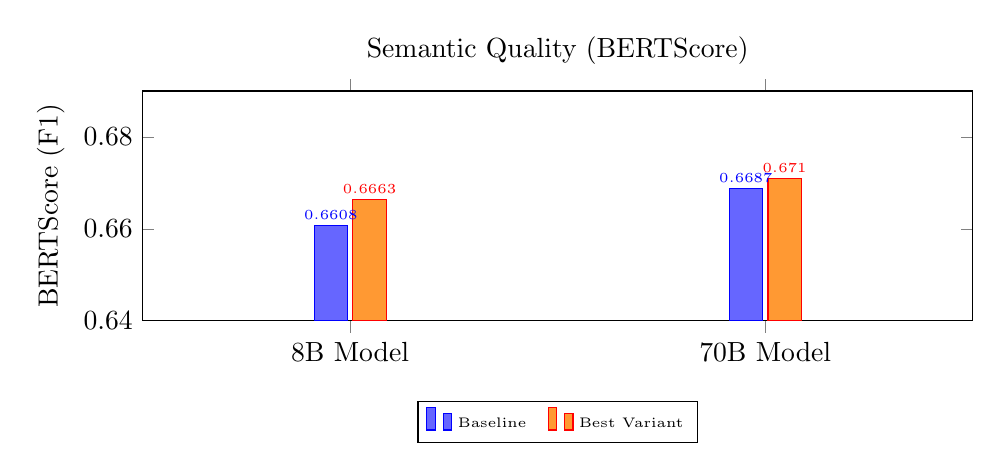
\begin{tikzpicture}
      \begin{axis}[
        ybar,
        % Adjust bar width for single column
        bar width=12pt, 
        % Set width to the line width (column width)
        width=\linewidth, 
        height=4.5cm, % Slightly reduced height to save vertical space
        symbolic x coords={8B Model,70B Model},
        xtick=data,
        % Adjust y-limits slightly for cleaner look
        ymin=0.64, ymax=0.69, 
        ylabel={BERTScore (F1)},
        title={Semantic Quality (BERTScore)},
        nodes near coords,
        every node near coord/.append style={
          font=\tiny, % Smaller font for values
          anchor=south,
          yshift=1pt,
          inner sep=1pt
        },
        nodes near coords style={
          /pgf/number format/fixed,
          /pgf/number format/precision=4
        },
        enlarge x limits=0.5,
        % Legend adjustment for narrow column
        legend style={
            at={(0.5,-0.35)},
            anchor=north,
            legend columns=2, 
            font=\tiny,
            /tikz/every even column/.append style={column sep=0.2cm}
        }
      ]
        \addplot+[fill=blue!60] coordinates {(8B Model,0.6608) (70B Model,0.6687)};
        \addplot+[fill=orange!80] coordinates {(8B Model,0.6663) (70B Model,0.6710)};
        \legend{Baseline, Best Variant}
      \end{axis}
    \end{tikzpicture}
  \end{subfigure}

  \vspace{2pt}

  % --- BARTScore ---
  \begin{subfigure}{\linewidth}
    \centering
    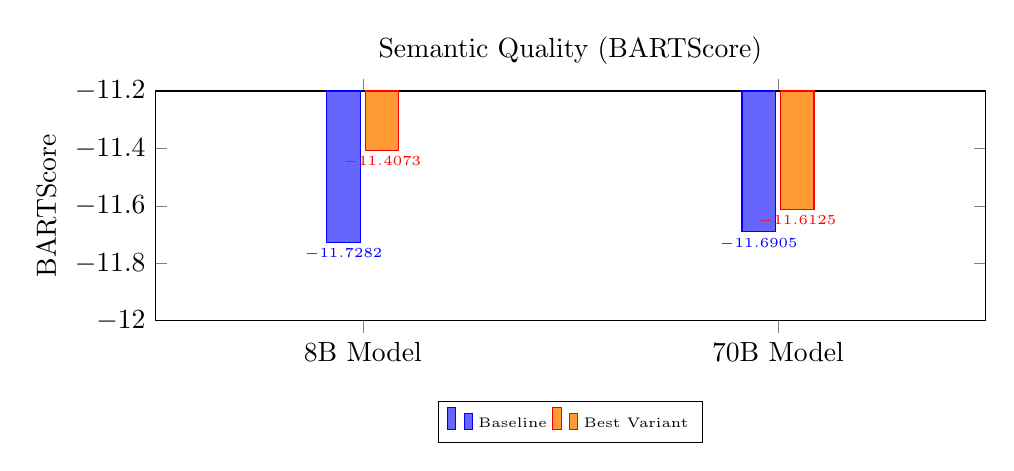
\begin{tikzpicture}
      \begin{axis}[
        ybar,
        bar width=12pt,
        width=\linewidth,
        height=4.5cm,
        symbolic x coords={8B Model,70B Model},
        xtick=data,
        % Adjusted y-limits for negative bars
        ymin=-12.0, ymax=-11.2, 
        ylabel={BARTScore},
        title={Semantic Quality (BARTScore)},
        nodes near coords,
        every node near coord/.append style={
          font=\tiny,
          anchor=north, % Labels below bar for negative values
          yshift=-1pt,
          inner sep=1pt
        },
        nodes near coords style={
          /pgf/number format/fixed,
          /pgf/number format/precision=4
        },
        enlarge x limits=0.5,
        legend style={
            at={(0.5,-0.35)},
            anchor=north,
            legend columns=2, 
            font=\tiny
        }
      ]
        \addplot+[fill=blue!60] coordinates {(8B Model,-11.7282) (70B Model,-11.6905)};
        \addplot+[fill=orange!80] coordinates {(8B Model,-11.4073) (70B Model,-11.6125)};
        \legend{Baseline, Best Variant}
      \end{axis}
    \end{tikzpicture}
  \end{subfigure}

  \vspace{2pt}

  % --- LLM-as-a-Judge ---
  \begin{subfigure}{\linewidth}
    \centering
    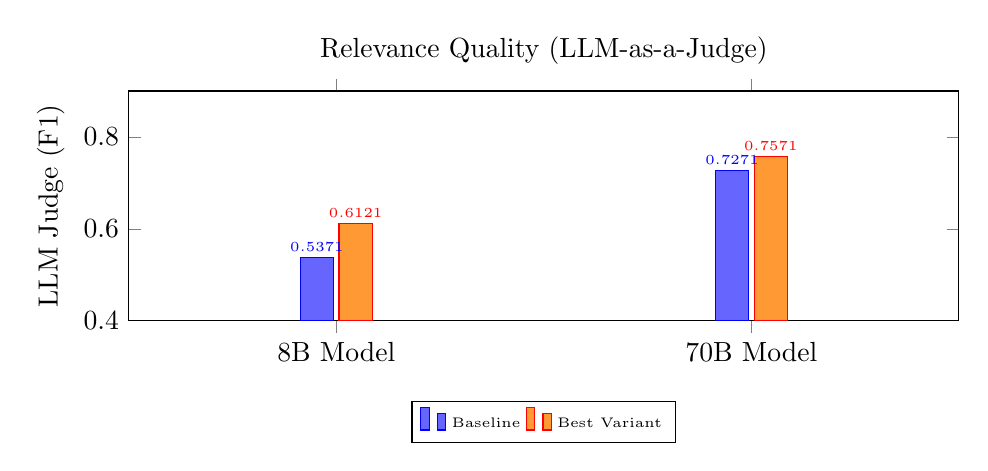
\begin{tikzpicture}
      \begin{axis}[
        ybar,
        bar width=12pt,
        width=\linewidth,
        height=4.5cm,
        symbolic x coords={8B Model,70B Model},
        xtick=data,
        ymin=0.4, ymax=0.9,
        ylabel={LLM Judge (F1)},
        title={Relevance Quality (LLM-as-a-Judge)},
        nodes near coords,
        every node near coord/.append style={
          font=\tiny,
          anchor=south,
          yshift=1pt,
          inner sep=1pt
        },
        nodes near coords style={
          /pgf/number format/fixed,
          /pgf/number format/precision=4
        },
        enlarge x limits=0.5,
        legend style={
            at={(0.5,-0.35)},
            anchor=north,
            legend columns=2, 
            font=\tiny
        }
      ]
        \addplot+[fill=blue!60] coordinates {(8B Model,0.5371) (70B Model,0.7271)};
        \addplot+[fill=orange!80] coordinates {(8B Model,0.6121) (70B Model,0.7571)};
        \legend{Baseline, Best Variant}
      \end{axis}
    \end{tikzpicture}
  \end{subfigure}

  \caption{Performance Comparison of 8B vs 70B Models across Different Evaluation Metrics.}
  \label{fig:pgfplots_bars}
\end{figure}

% \begin{figure}[H]
%   \centering
%   % --- BERTScore (positif: label di atas batang) ---
%   \begin{subfigure}{0.9\textwidth}
%     \centering
%     \begin{tikzpicture}
%       \begin{axis}[
%         ybar,
%         bar width=18pt,
%         width=\textwidth,
%         height=5cm,
%         symbolic x coords={8B Model,70B Model},
%         xtick=data,
%         ymin=0.65,ymax=0.68,
%         ylabel={BERTScore (F1)},
%         title={Perbandingan Kualitas Semantik (BERTScore)},
%         nodes near coords,
%         every node near coord/.append style={
%           font=\scriptsize,
%           anchor=south,   % label di atas batang
%           yshift=2pt,     % geser sedikit ke atas
%           inner sep=1pt
%         },
%         nodes near coords style={
%           /pgf/number format/fixed,
%           /pgf/number format/precision=4
%         },
%         enlarge x limits=0.4,
%         legend style={at={(0.5,-0.25)},anchor=north,legend columns=2}
%       ]
%         \addplot+[fill=blue!60] coordinates {(8B Model,0.6608) (70B Model,0.6687)};
%         \addplot+[fill=orange!80] coordinates {(8B Model,0.6663) (70B Model,0.6710)};
%         \legend{Baseline, Best Variant (ReAct+LA / Lis Materi)}
%       \end{axis}
%     \end{tikzpicture}
%   \end{subfigure}

%   \vspace{6pt}

%   % --- BARTScore (negatif: gunakan anchor=north dan yshift negatif) ---
%   \begin{subfigure}{0.9\textwidth}
%     \centering
%     \begin{tikzpicture}
%       \begin{axis}[
%         ybar,
%         bar width=18pt,
%         width=\textwidth,
%         height=5cm,
%         symbolic x coords={8B Model,70B Model},
%         xtick=data,
%         ymin=-11.9,ymax=-11.3,
%         ylabel={BARTScore},
%         title={Perbandingan Kualitas Semantik (BARTScore)},
%         nodes near coords,
%         every node near coord/.append style={
%           font=\scriptsize,
%           anchor=north,  % untuk batang negatif, anchor ke utara (agar label "di atas" batang)
%           yshift=-2pt,   % geser sedikit ke atas relatif ke batang negatif
%           inner sep=1pt
%         },
%         nodes near coords style={
%           /pgf/number format/fixed,
%           /pgf/number format/precision=4
%         },
%         enlarge x limits=0.4,
%         legend style={at={(0.5,-0.25)},anchor=north,legend columns=2}
%       ]
%         \addplot+[fill=blue!60] coordinates {(8B Model,-11.7282) (70B Model,-11.6905)};
%         \addplot+[fill=orange!80] coordinates {(8B Model,-11.4073) (70B Model,-11.6125)};
%         \legend{Baseline, Best Variant (ReAct+LA / Lis Materi)}
%       \end{axis}
%     \end{tikzpicture}
%   \end{subfigure}

%   \vspace{6pt}

%   % --- LLM-as-a-Judge (positif: label di atas batang) ---
%   \begin{subfigure}{0.9\textwidth}
%     \centering
%     \begin{tikzpicture}
%       \begin{axis}[
%         ybar,
%         bar width=18pt,
%         width=\textwidth,
%         height=5cm,
%         symbolic x coords={8B Model,70B Model},
%         xtick=data,
%         ymin=0.5,ymax=0.8,
%         ylabel={LLM-as-a-Judge (F1)},
%         title={Perbandingan Kualitas Relevansi (LLM-as-a-Judge)},
%         nodes near coords,
%         every node near coord/.append style={
%           font=\scriptsize,
%           anchor=south,   % label di atas batang
%           yshift=2pt,     % geser sedikit ke atas
%           inner sep=1pt
%         },
%         nodes near coords style={
%           /pgf/number format/fixed,
%           /pgf/number format/precision=4
%         },
%         enlarge x limits=0.4,
%         legend style={at={(0.5,-0.25)},anchor=north,legend columns=2}
%       ]
%         \addplot+[fill=blue!60] coordinates {(8B Model,0.5371) (70B Model,0.7271)};
%         \addplot+[fill=orange!80] coordinates {(8B Model,0.6121) (70B Model,0.7571)};
%         \legend{Baseline, Best Variant (ReAct+LA / Lis Materi)}
%       \end{axis}
%     \end{tikzpicture}
%   \end{subfigure}

%   \caption{Perbandingan Kinerja Model 8B vs 70B pada metrik evaluasi berbeda.}
%   \label{fig:pgfplots_bars}
% \end{figure}
% \begin{figure}[htbp]
% \centering
% % Placeholder for the actual image file from your source
% \includegraphics[width=\columnwidth]{contents/chapter-4/fig\_comparison\_8b_70b.png}
% \caption{Performance Comparison of 8B vs 70B Models across Different Evaluation Metrics (Baseline vs. Best Variant)}
% \label{fig:model_performance}
% \end{figure}

The validation by human experts confirms the potential of the system, with the best-performing model (Llama 3.1 8B with ReAct plus LA) being rated as "Usable with minor revision." Experts assessed the feedback, motivation, and appreciation aspects positively, as detailed in Tables \ref{tab:expert_feedback}, \ref{tab:expert_motivation}, and \ref{tab:expert_appreciation}.

\begin{table}[htbp]
\caption{Expert Assessment on Feedback Quality Aspects}
\centering
\scriptsize
\begin{tabular}{|l|l|c|}
\hline
\textbf{Indicator} & \textbf{Question} & \textbf{Score} \\ \hline
F1 (Clarity) & Feedback is easy to understand. & 4 \\ \hline
F2 (Specificity) & Feedback gives specific suggestions. & 4 \\ \hline
F3 (Relevance) & Feedback fits the learning activity. & 3 \\ \hline
F4 (Constructiveness) & Feedback helps fix errors. & 4 \\ \hline
F5 (Feed-forward) & Feedback provides next steps. & 4 \\ \hline
\end{tabular}
\label{tab:expert_feedback}
\end{table}

\begin{table}[htbp]
\caption{Expert Assessment on Motivational Support Aspects}
\centering
\scriptsize
\begin{tabular}{|l|l|c|}
\hline
\textbf{Indicator} & \textbf{Question} & \textbf{Score} \\ \hline
M1 (Intrinsic Drive) & Makes me more excited to learn. & 4 \\ \hline
M2 (Goal Drive) & Helps stay focused on learning goals. & 5 \\ \hline
M3 (Autonomy) & Gives freedom in learning methods. & 4 \\ \hline
M4 (Competence) & Makes me feel more confident. & 4 \\ \hline
M5 (Relatedness) & Support feels empathetic. & 3 \\ \hline
\end{tabular}
\label{tab:expert_motivation}
\end{table}

\begin{table}[htbp]
\caption{Expert Assessment on Appreciation and Emotional Support}
\centering
\scriptsize
\begin{tabular}{|l|l|c|}
\hline
\textbf{Indicator} & \textbf{Question} & \textbf{Score} \\ \hline
A1 (Effort Recog.) & Appreciates effort, not just results. & 5 \\ \hline
A2 (Proportional) & Praise feels sincere and appropriate. & 3 \\ \hline
A3 (Confidence) & Appreciation boosts confidence. & 4 \\ \hline
A4 (Emotional Supp.) & Provides calming responses. & 4 \\ \hline
A5 (Positive Reinf.) & Language makes me feel valued. & 3 \\ \hline
\end{tabular}
\label{tab:expert_appreciation}
\end{table}

Experts noted areas for improvement such as the need for more specific context references and a less robotic tone in motivational support. These findings also reinforce the evaluation of prompt quality based on the theory-driven prompt manual, where a high prompt score does not necessarily guarantee optimal model output without considering model size and capabilities \cite{jacobsen2025promises}. The feedback was deemed effective in maintaining focus on learning goals although it sometimes lacked the empathetic connection found in human interaction.

\section{Conclusions}
This study conducted experiments to design improve and evaluate the quality of pedagogical feedback generated by LLMs focusing on enhancing feedback motivation and appreciation to support student Self Regulated Learning. The improvement was achieved through context engineering methods enriched with learning analytics extracted from synthetic student Kanban board data without fine tuning the models. Based on the analysis the following conclusions are drawn to address the research questions.

First the method of context engineering combined with learning analytics proved successful in improving LLM feedback quality compared to the Baseline although its effectiveness depended heavily on the model size. For the small model Llama 3.1 8B the addition of complex context involving ReAct and learning analytics consistently provided the highest performance improvements across all quantitative metrics. This indicates that small models benefit significantly from rich and structured context guidance to produce feedback that is more relevant and of higher semantic quality.

Second model size has a significant and bidirectional influence on feedback quality. The large model Llama 3.3 70B showed far superior Baseline performance compared to the 8B model particularly in terms of relevance. However the 70B model did not benefit from complex contexts achieving its best performance with simpler contexts such as the Material List. The addition of complex ReAct and LA contexts even degraded its performance likely because the prompt overly constrained the large model forcing it to mimic the descriptive style of the small model rather than approaching the ground truth.

Third based on human expert perception the feedback generated by the best performing model Llama 3.1 8B with ReAct and LA was declared Usable with minor revision. Experts confirmed the potential of the chatbot as an accessible scaffolding system. Suggested revisions focused on adjusting language tonality eliminating negative diction addressing response category overlap improving feedback specificity and increasing the variation of motivational responses. These findings also emphasize that a good score from a theory driven prompt manual does not necessarily guarantee optimal model output without considering other factors like model size and language capabilities.

In conclusion this research determines that context engineering enriched with learning analytics is an effective practical and computationally efficient strategy for improving pedagogical feedback especially when applied to small LLM models.


\section{Future Works}
Based on the limitations and potential developments identified in this study future research can consider several advancements to further enhance the quality and applicability of pedagogical feedback agents.

First further investigation is needed regarding the influence of complex context engineering on large LLMs to understand their boundaries and characteristics in responding to rich contexts. Understanding why larger models may degrade with complex prompting is crucial for optimizing their use in educational settings.

Second developing human expert evaluation using A B testing is recommended where experts assess two feedback variations to directly select the best one allowing for a more comparative and definitive assessment of quality.

Third experiments should include more diverse prompt variations including those adjusting language tonality according to user demographic characteristics to improve the empathetic connection and relevance perceived by students.

Fourth further research is required to identify optimal prompts for generating high quality feedback going beyond assessments based solely on theory driven prompt manuals. This involves exploring prompt structures that yield the best empirical results rather than just theoretical compliance.

Fifth conducting statistical hypothesis testing is essential to strengthen the validity of quantitative findings and evolve the current exploratory direction into robust hypotheses.

Sixth evaluating LLMs with superior Indonesian language performance is suggested to observe the impact on feedback quality as language proficiency significantly affects the nuance and accuracy of pedagogical responses.

Finally using real student learning data to extract learning analytics and involving a larger number of experts for validation and ground truth collection will enhance the accuracy and relevance of research results ensuring the system is robust for real world application.

% This chapter presents the results and analysis of the experiments which were conducted by implementing the improvement methods divided into two main stages context engineering and Learning Analytics followed by the creation of specific prompt variations. The experiments utilized synthetic student datasets processed through four distinct prompt variations including Baseline Material List Learning Analytics and ReAct plus Learning Analytics on two LLM models Llama 3.1 8B and Llama 3.3 70B.

% The comparative analysis of feedback improvement methods reveals distinct performance patterns dependent on model size and context complexity. Quantitative evaluation using BERTScore and BARTScore indicates that the smaller 8B model achieved the most significant quality improvement when integrating complex context engineering and Learning Analytics specifically the ReAct plus LA variation. This suggests that smaller models rely heavily on structured guidance to enhance semantic quality \cite{tang2025fewshot, pawlik2025choice}. Conversely the larger 70B model demonstrated optimal performance with simpler context engineering such as the Material List variation while complex contexts like ReAct plus LA tended to stagnate or degrade its performance \cite{tang2025fewshot, pawlik2025choice}.

% Regarding the influence of model size the analysis shows that the 70B model possesses a superior baseline capacity compared to the 8B model particularly in relevance metrics measured by LLM as a Judge. However the 8B model exhibited higher responsiveness to context engineering interventions. Qualitative analysis highlights that the 70B model generates more prescriptive and linguistically varied feedback whereas the 8B model tends to be descriptive and repetitive often failing to separate appreciation from critique.

% The validation by human experts confirms the potential of the system with the best performing model Llama 3.1 8B with ReAct plus LA being rated as Usable with minor revision. Experts assessed the feedback motivation and appreciation aspects positively but noted areas for improvement such as the need for more specific context references and a less robotic tone in motivational support. These findings also reinforce the evaluation of prompt quality based on the theory-driven prompt manual, where a high prompt score does not necessarily guarantee optimal model output without considering model size and capabilities \cite{jacobsen2025promises}. The feedback was deemed effective in maintaining focus on learning goals although it sometimes lacked the empathetic connection found in human interaction.

% Number equations consecutively. To make your 
% equations more compact, you may use the solidus (~/~), the exp function, or 
% appropriate exponents. Italicize Roman symbols for quantities and variables, 
% but not Greek symbols. Use a long dash rather than a hyphen for a minus 
% sign. Punctuate equations with commas or periods when they are part of a 
% sentence, as in:

% Be sure that the 
% symbols in your equation have been defined before or immediately following 
% the equation. Use ``\eqref{eq}'', not ``Eq.~\eqref{eq}'' or ``equation \eqref{eq}'', except at 
% the beginning of a sentence: ``Equation \eqref{eq} is . . .''

% \subsection{\LaTeX-Specific Advice}

% Please use ``soft'' (e.g., \verb|\eqref{Eq}|) cross references instead
% of ``hard'' references (e.g., \verb|(1)|). That will make it possible
% to combine sections, add equations, or change the order of figures or
% citations without having to go through the file line by line.

% Please don't use the \verb|{eqnarray}| equation environment. Use
% \verb|{align}| or \verb|{IEEEeqnarray}| instead. The \verb|{eqnarray}|
% environment leaves unsightly spaces around relation symbols.

% Please note that the \verb|{subequations}| environment in {\LaTeX}
% will increment the main equation counter even when there are no
% equation numbers displayed. If you forget that, you might write an
% article in which the equation numbers skip from (17) to (20), causing
% the copy editors to wonder if you've discovered a new method of
% counting.

% {\BibTeX} does not work by magic. It doesn't get the bibliographic
% data from thin air but from .bib files. If you use {\BibTeX} to produce a
% bibliography you must send the .bib files. 

% {\LaTeX} can't read your mind. If you assign the same label to a
% subsubsection and a table, you might find that Table I has been cross
% referenced as Table IV-B3. 

% {\LaTeX} does not have precognitive abilities. If you put a
% \verb|\label| command before the command that updates the counter it's
% supposed to be using, the label will pick up the last counter to be
% cross referenced instead. In particular, a \verb|\label| command
% should not go before the caption of a figure or a table.

% Do not use \verb|\nonumber| inside the \verb|{array}| environment. It
% will not stop equation numbers inside \verb|{array}| (there won't be
% any anyway) and it might stop a wanted equation number in the
% surrounding equation.

% \subsection{Some Common Mistakes}\label{SCM}
% \begin{itemize}
% \item The word ``data'' is plural, not singular.
% \item The subscript for the permeability of vacuum $\mu_{0}$, and other common scientific constants, is zero with subscript formatting, not a lowercase letter ``o''.
% \item In American English, commas, semicolons, periods, question and exclamation marks are located within quotation marks only when a complete thought or name is cited, such as a title or full quotation. When quotation marks are used, instead of a bold or italic typeface, to highlight a word or phrase, punctuation should appear outside of the quotation marks. A parenthetical phrase or statement at the end of a sentence is punctuated outside of the closing parenthesis (like this). (A parenthetical sentence is punctuated within the parentheses.)
% \item A graph within a graph is an ``inset'', not an ``insert''. The word alternatively is preferred to the word ``alternately'' (unless you really mean something that alternates).
% \item Do not use the word ``essentially'' to mean ``approximately'' or ``effectively''.
% \item In your paper title, if the words ``that uses'' can accurately replace the word ``using'', capitalize the ``u''; if not, keep using lower-cased.
% \item Be aware of the different meanings of the homophones ``affect'' and ``effect'', ``complement'' and ``compliment'', ``discreet'' and ``discrete'', ``principal'' and ``principle''.
% \item Do not confuse ``imply'' and ``infer''.
% \item The prefix ``non'' is not a word; it should be joined to the word it modifies, usually without a hyphen.
% \item There is no period after the ``et'' in the Latin abbreviation ``et al.''.
% \item The abbreviation ``i.e.'' means ``that is'', and the abbreviation ``e.g.'' means ``for example''.
% \end{itemize}
% An excellent style manual for science writers is \cite{b7}.

% \subsection{Authors and Affiliations}
% \textbf{The class file is designed for, but not limited to, six authors.} A 
% minimum of one author is required for all conference articles. Author names 
% should be listed starting from left to right and then moving down to the 
% next line. This is the author sequence that will be used in future citations 
% and by indexing services. Names should not be listed in columns nor group by 
% affiliation. Please keep your affiliations as succinct as possible (for 
% example, do not differentiate among departments of the same organization).

% \subsection{Identify the Headings}
% Headings, or heads, are organizational devices that guide the reader through 
% your paper. There are two types: component heads and text heads.

% Component heads identify the different components of your paper and are not 
% topically subordinate to each other. Examples include Acknowledgments and 
% References and, for these, the correct style to use is ``Heading 5''. Use 
% ``figure caption'' for your Figure captions, and ``table head'' for your 
% table title. Run-in heads, such as ``Abstract'', will require you to apply a 
% style (in this case, italic) in addition to the style provided by the drop 
% down menu to differentiate the head from the text.

% Text heads organize the topics on a relational, hierarchical basis. For 
% example, the paper title is the primary text head because all subsequent 
% material relates and elaborates on this one topic. If there are two or more 
% sub-topics, the next level head (uppercase Roman numerals) should be used 
% and, conversely, if there are not at least two sub-topics, then no subheads 
% should be introduced.

% \subsection{Figures and Tables}
% \paragraph{Positioning Figures and Tables} Place figures and tables at the top and 
% bottom of columns. Avoid placing them in the middle of columns. Large 
% figures and tables may span across both columns. Figure captions should be 
% below the figures; table heads should appear above the tables. Insert 
% figures and tables after they are cited in the text. Use the abbreviation 
% ``Fig.~\ref{fig}'', even at the beginning of a sentence.

% \begin{table}[htbp]
% \caption{Table Type Styles}
% \begin{center}
% \begin{tabular}{|c|c|c|c|}
% \hline
% \textbf{Table}&\multicolumn{3}{|c|}{\textbf{Table Column Head}} \\
% \cline{2-4} 
% \textbf{Head} & \textbf{\textit{Table column subhead}}& \textbf{\textit{Subhead}}& \textbf{\textit{Subhead}} \\
% \hline
% copy& More table copy$^{\mathrm{a}}$& &  \\
% \hline
% \multicolumn{4}{l}{$^{\mathrm{a}}$Sample of a Table footnote.}
% \end{tabular}
% \label{tab1}
% \end{center}
% \end{table}

% \begin{figure}[htbp]
% \centerline{\includegraphics{fig1.png}}
% \caption{Example of a figure caption.}
% \label{fig}
% \end{figure}

% Figure Labels: Use 8 point Times New Roman for Figure labels. Use words 
% rather than symbols or abbreviations when writing Figure axis labels to 
% avoid confusing the reader. As an example, write the quantity 
% ``Magnetization'', or ``Magnetization, M'', not just ``M''. If including 
% units in the label, present them within parentheses. Do not label axes only 
% with units. In the example, write ``Magnetization (A/m)'' or ``Magnetization 
% \{A[m(1)]\}'', not just ``A/m''. Do not label axes with a ratio of 
% quantities and units. For example, write ``Temperature (K)'', not 
% ``Temperature/K''.

% \section*{Acknowledgment}

% The preferred spelling of the word ``acknowledgment'' in America is without 
% an ``e'' after the ``g''. Avoid the stilted expression ``one of us (R. B. 
% G.) thanks $\ldots$''. Instead, try ``R. B. G. thanks$\ldots$''. Put sponsor 
% acknowledgments in the unnumbered footnote on the first page.

% \section*{References}

% Please cite all your references \cite{2023Bhawal-SST},\cite{2023Chen-Phase-Shift-DAB}. References are stored in a bibtex file "references.bib". You can use Mendeley or Jabref for your reference manager. 

%Please number citations consecutively within brackets \cite{b1}. The 
%sentence punctuation follows the bracket \cite{b2}. Refer simply to the reference 
%number, as in \cite{b3}---do not use ``Ref. \cite{b3}'' or ``reference \cite{b3}'' except at 
%the beginning of a sentence: ``Reference \cite{b3} was the first $\ldots$''
%
%Number footnotes separately in superscripts. Place the actual footnote at 
%the bottom of the column in which it was cited. Do not put footnotes in the 
%abstract or reference list. Use letters for table footnotes.
%
%Unless there are six authors or more give all authors' names; do not use 
%``et al.''. Papers that have not been published, even if they have been 
%submitted for publication, should be cited as ``unpublished'' \cite{b4}. Papers 
%that have been accepted for publication should be cited as ``in press'' \cite{b5}. 
%Capitalize only the first word in a paper title, except for proper nouns and 
%element symbols.
%
%For papers published in translation journals, please give the English 
%citation first, followed by the original foreign-language citation \cite{b6}.



\bibliography{references}{}
\bibliographystyle{IEEEtran}

%\begin{thebibliography}{00}
%\bibitem{b1} G. Eason, B. Noble, and I. N. Sneddon, ``On certain integrals of Lipschitz-Hankel type involving products of Bessel functions,'' Phil. Trans. Roy. Soc. London, vol. A247, pp. 529--551, April 1955.
%\bibitem{b2} J. Clerk Maxwell, A Treatise on Electricity and Magnetism, 3rd ed., vol. 2. Oxford: Clarendon, 1892, pp.68--73.
%\bibitem{b3} I. S. Jacobs and C. P. Bean, ``Fine particles, thin films and exchange anisotropy,'' in Magnetism, vol. III, G. T. Rado and H. Suhl, Eds. New York: Academic, 1963, pp. 271--350.
%\bibitem{b4} K. Elissa, ``Title of paper if known,'' unpublished.
%\bibitem{b5} R. Nicole, ``Title of paper with only first word capitalized,'' J. Name Stand. Abbrev., in press.
%\bibitem{b6} Y. Yorozu, M. Hirano, K. Oka, and Y. Tagawa, ``Electron spectroscopy studies on magneto-optical media and plastic substrate interface,'' IEEE Transl. J. Magn. Japan, vol. 2, pp. 740--741, August 1987 [Digests 9th Annual Conf. Magnetics Japan, p. 301, 1982].
%\bibitem{b7} M. Young, The Technical Writer's Handbook. Mill Valley, CA: University Science, 1989.
%\end{thebibliography}



\end{document}
